\section{Алгоритмы и структуры данных}
\subsection{Преобразование цветового пространства (RGB → YCbCr)}

Перед сжатием изображений в формате JPEG зачастую используется преобразование из цветового пространства RGB в YCbCr. 
Это обусловлено как особенностями восприятия цвета человеком, так и требованиями алгоритмов сжатия.


Такое разделение позволяет применить хрома-субдискретизацию — уменьшение разрешения цветовых компонент — без заметного ухудшения качества изображения.
Для RGB с диапазоном значений от 0 до 255, преобразование в YCbCr выполняется по следующим формулам:


\begin{equation}
    \begin{aligned}
        Y &= 0.299R + 0.587G + 0.114B; \\
        Cb &= -0.168736R - 0.331264G + 0.5B + 128; \\
        Cr &= 0.5R - 0.418688G - 0.081312B + 128.
    \end{aligned}
\end{equation}

Каждое из этих вычислений требует константного числа операций (умножений и сложений).
Поскольку обработка всех пикселей независима, общее время работы линейно зависит от их количества $O(n)$.

Здесь значения R, G, B принимаются в диапазоне $[0, 255]$. 
Смещение на 128 единиц в формулах для Cb и Cr необходимо для корректного представления как положительных, так и отрицательных значений в беззнаковом формате (unsigned int).

Поскольку компоненты Cb и Cr менее значимы для восприятия, их можно хранить с пониженным разрешением. 
Наиболее распространённый формат — 4:2:0, при котором на каждые 4 пикселя хранится 4 значения яркости Y и по 1 значению Cb и Cr. 
Это даёт значительное уменьшение объёма данных без существенного ущерба для качества изображения.



\subsubsection{Преимущества YCbCr}
    \begin{itemize}
        \item Дает возможность сжатия на уровне разрешения без видимых потерь качества;
        \item Разделение яркости и цвета позволяет применять различные методы компрессии к компонентам Y и CbCr;
        \item Поддерживается большинством стандартов обработки изображений и видео.
    \end{itemize}

    Таким образом, преобразование RGB → YCbCr является ключевым шагом в JPEG и других алгоритмах сжатия, 
    позволяющим использовать особенности восприятия цвета человеком для достижения более высокой степени сжатия.



%%%%%%%%%%%%%%%%%%%%%%%%%%%%%%%%%%%%%%%%%%%%%%%
\subsection{Субдискретизация}
На втором этапе сжатия изображения применяется методика, известная как субдискретизация цветности (англ. chroma subsampling). 
Её ключевая идея заключается в сокращении объёма данных, содержащих информацию о цвете, путём уменьшения пространственного разрешения цветовых компонентов. 
Это возможно благодаря физиологической особенности зрительной системы человека: 
она в гораздо большей степени чувствительна к деталям яркости (компонент Y — luminance), чем к изменениям цветовых оттенков (компоненты Cb и Cr — chrominance).

В практической реализации данный метод означает, что цветовая информация (Cr и Cb) кодируется с меньшей точностью по сравнению с яркостной. 
Существует несколько вариантов схем хрома-субдискретизации, которые различаются по степени уменьшения разрешения цветовых компонентов:

4:4:4 — нет сжатия, все компоненты Y, Cb и Cr сохраняют оригинальное разрешение.

4:2:2 — разрешение Cb и Cr уменьшается в два раза по сравнению с Y.

4:2:0 — стандарт для большинства сжатых форматов, где разрешение Cb и Cr уменьшается в два раза как по вертикали, так и по горизонтали.

Схема 4:2:0 является наиболее распространенной для видео и изображений, так как она дает хороший баланс между качеством и сжатием. 
Она предполагает, что на каждые четыре пикселя яркости (расположенных в виде блока 2×2) приходится всего один усреднённый пиксел Cr и один усреднённый пиксел Cb. 
То есть цветовые значения вычисляются как средние значения для группы пикселей, и это значение применяется ко всей группе. 
В результате разрешение цветовых компонентов уменьшается в четыре раза (на 75\%) по сравнению с яркостной компонентой.

Для визуализации можно представить исходное изображение как состоящее из трёх равнозначных слоёв:

Y (яркость),

Cb (синий цветовой компонент),

Cr (красный цветовой компонент).

До субдискретизации каждый из этих компонентов имел одинаковое разрешение и соответственно одинаковый вклад в общий объём данных:


\begin{equation}
    Y + Cb + Cr = 1+1+1=3 \text{ единицы информации}.
\end{equation}

После применения схемы 4:2:0, каждая из цветовых компонент уменьшается до $\frac{1}{4}$ исходного размера, а яркостная остаётся без изменений:

\begin{equation}
    Y + \frac{1}{4}Cb + \frac{1}{4}Cr = 1 + 0.25 + 0.25 = 1.5 \text{ единицы информации}.
\end{equation}

\begin{figure}[H]
    \centering
    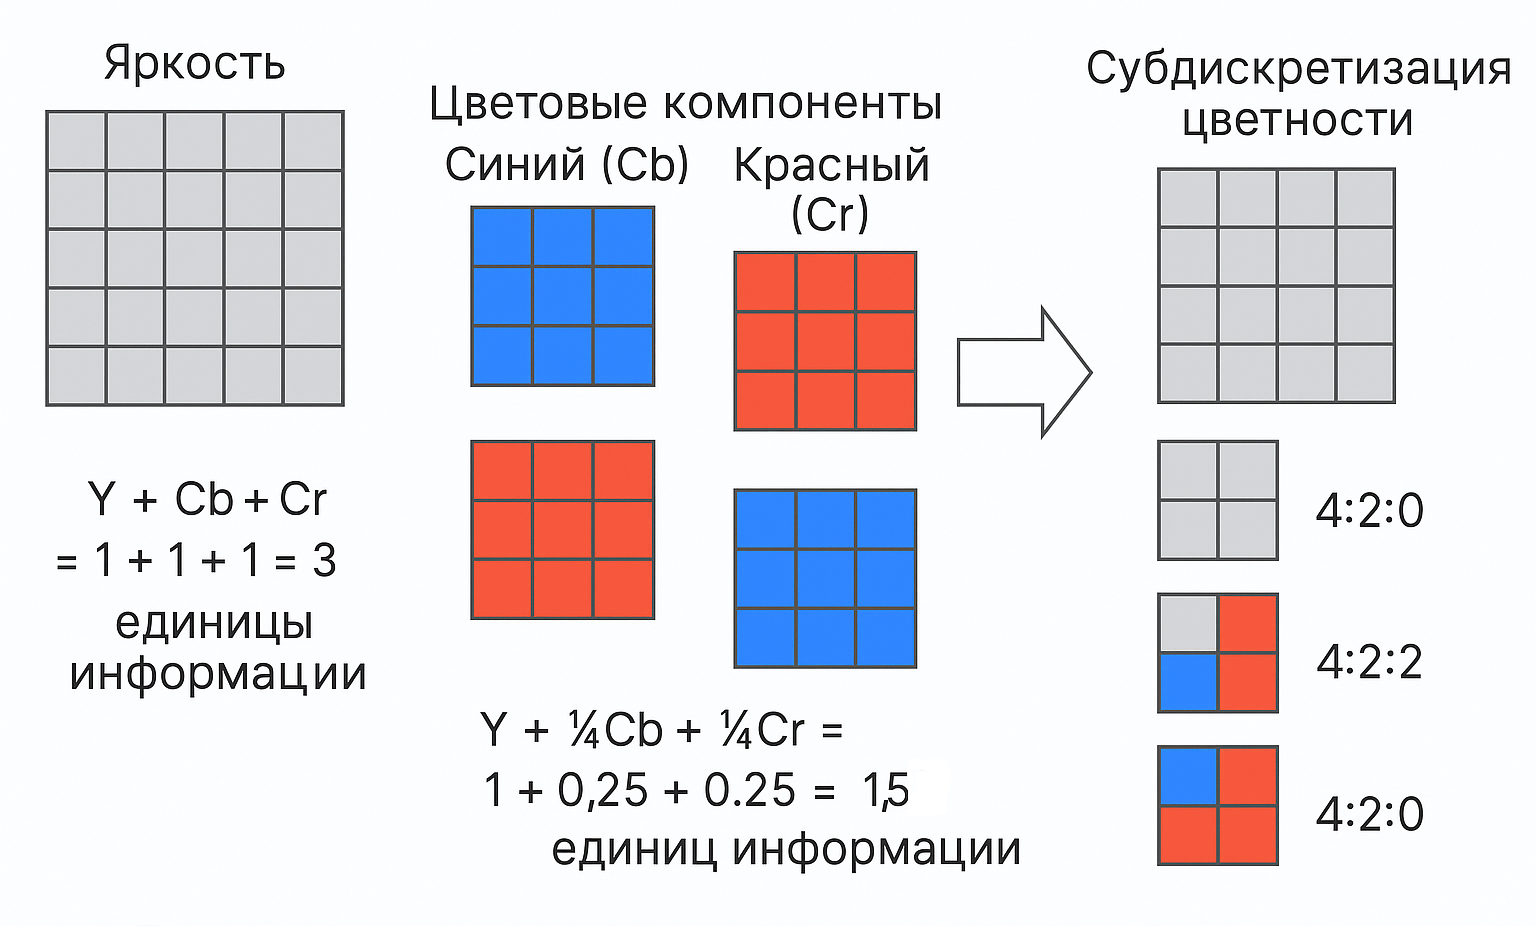
\includegraphics[width=0.7\textwidth]{/home/evgen/Coursework/app/diplom/images/sub_discretization1.png}
    \caption{Как происходит преобразование}
    \label{fig:sub_dis}
\end{figure}

Таким образом, достигается двукратное уменьшение общего объёма данных, подлежащих хранению или передаче.

Что важно, такое преобразование происходит практически без визуальных потерь качества. 
Несмотря на то, что цветовые данные редуцируются, человеческий глаз практически не воспринимает различие между оригинальным и сжатым изображением. 
Именно поэтому субдискретизация цветности широко применяется в большинстве алгоритмов сжатия изображений и видео (JPEG, MPEG, H.264),
где критически важно достичь компромисса между качеством и эффективностью хранения данных.

%%%%%%%%%%%%%%%%%%%%%%%%%%%%%%%%%%%%%%%%%%%%%
\subsection{Дискретное косинус-преобразование}

После преобразования изображения из цветового пространства RGB в YCbCr и выполнения хрома-субдискретизации (уменьшения разрешения цветовых компонент Cb и Cr), 
выполняется разбиение изображения на блоки фиксированного размера 8×8 пикселей. 
Однако размеры исходного изображения не всегда кратны восьми, что делает невозможным непосредственное и равномерное разбиение без остатка. 
В таких случаях производится предварительная корректировка размеров изображения: вычисляется необходимое количество дополнительных строк и столбцов, 
которые должны быть добавлены к правому и нижнему краю изображения для достижения кратности 8.

Добавление недостающих строк и столбцов осуществляется с помощью повторения граничных значений (пикселей) изображения, 
чтобы минимизировать искажения, возникающие на краях. 

\AddedBlocks

Этот шаг реализуется при помощи библиотеки OpenCV, предоставляющей функцию для симметричного дополнения изображений. 
После этого скорректированное изображение разбивается на непересекающиеся блоки размером 8×8.

\begin{figure}[H]
    \centering
    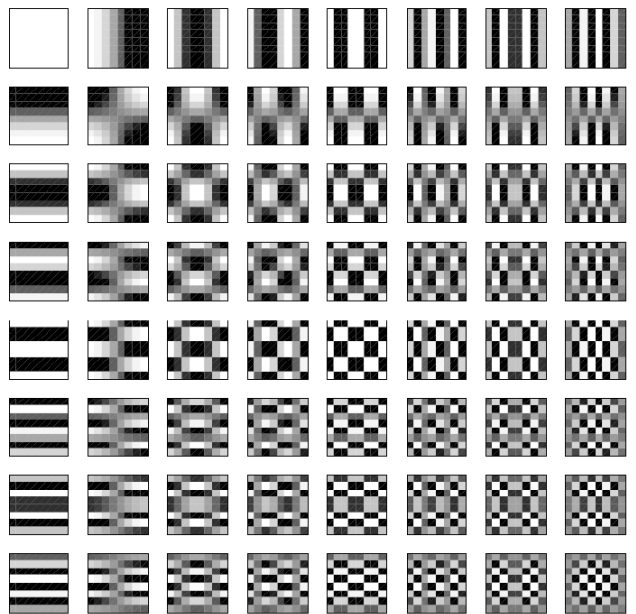
\includegraphics[width=0.7\textwidth]{/home/evgen/Coursework/app/diplom/images/bloks.png}
    \caption{Блоки 8х8}
    \label{fig:blocks}
\end{figure}


Для удобства хранения и последующей обработки эти блоки сохраняются в виде многомерных массивов с использованием библиотеки NumPy. 
Это позволяет эффективно обращаться к отдельным блокам, выполнять над ними математические преобразования и организовать дальнейший процесс.


Это важный шаг, позволяющий значительно повысить эффективность сжатия. 
Разделение на небольшие блоки позволяет применять алгоритмы сжатия локально, что упрощает обработку и улучшает степень компрессии.

Дальнейшая задача заключается в оценке уровня детализации внутри каждого блока. 
Если блок содержит мало визуальных деталей, его можно закодировать с меньшим числом битов, минимизируя потери качества. 
Для анализа степени детализации и выделения значимых компонент используется дискретное косинусное преобразование (ДКП, англ. Discrete Cosine Transform, DCT). 
Преобразование позволяет перейти от пространственного представления блока к частотному, выявляя частотные составляющие, которые имеют наибольшее значение для визуального восприятия.

Для понимания принципов работы ДКП целесообразно сначала рассмотреть его одномерную (векторную) форму, 
поскольку она обладает большей наглядностью и сохраняет все ключевые идеи, лежащие в основе двумерного варианта, применяемого в обработке изображений.


На рисунке~\ref{fig:coswaves}  показано восемь волн косинуса, $\omega(f) = \cos{(f \Theta)}$, при $0 \leq \Theta \leq \pi$ с частотами $f=0,1,\ldots,7$.

\begin{figure}[h!]
    \centering
    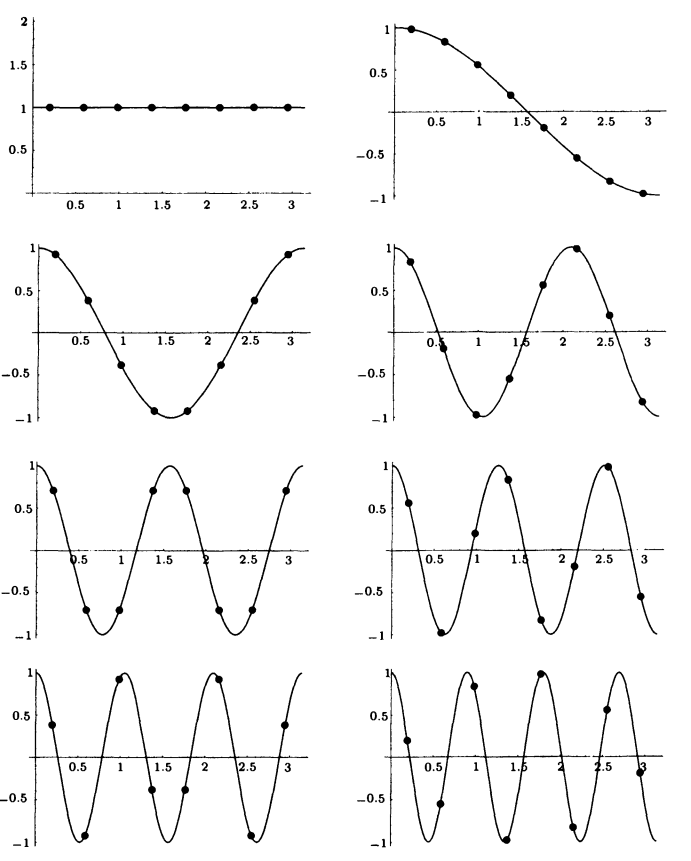
\includegraphics[width=0.7\textwidth]{/home/evgen/Coursework/app/diplom/images/basis_dct.png}
    \caption{Графики функций $\omega(f) = \cos{(f \Theta)}$ для различных частот $f$.}
    \label{fig:coswaves}
\end{figure}

На каждом графике отмечено восемь значений функции $\omega(f)$ с абс­циссами

\begin{equation}
    \Theta = \frac{\pi}{16}, 
                \frac{3\pi}{16}, 
                \frac{5\pi}{16}, 
                \frac{7\pi}{16}, 
                \frac{9\pi}{16}, 
                \frac{11\pi}{16}, 
                \frac{13\pi}{16}, 
                \frac{15\pi}{16}
    \label{eq:theta_values}
\end{equation}


которые формируют базисный вектор $v_f$. В результате получится восемь векторов $v_f, f = 0, 1, \dots, 7$ (всего 64 числа).

\clearpage
\BasisDCT

Они служат базисом одномерного косинусного преобразования, причём частота смены знаков увеличивается по строкам.

Можно показать, что все векторы $v_i$ ортогональны между со­бой (из-за специального выбора восьми точек отсчета $\Theta$). 
То же самое можно обнаружить прямым вычислением с помощью подхо­дящей математической программы. 
Значит, эти восемь векторов можно поместить в матрицу размером 8 на 8 и рассмотреть соот­ветствующее ей ортогональное преобразование - 
вращение в вось­мимерном пространстве, которое называется одномерным дискрет­ным косинус-преобразованием (DCT). 
% Двумерное DCT можно так­же интерпретировать как двойное вращение.////////////////////////////////////////////

Одномерное преобразование косинусов Дискретное (DCT) можно интерпретировать как представление вектора в базисе, состоящем из векторов $v_i$
В этом контексте любой вектор $p$ из соответствующего векторного пространства может быть выражен через линейную комбинацию этих базисных векторов $v_j$.


Например, выберем 8 (коррелированных) чисел $p=(0.6, 0.5, 0.4, 0.5, 0.6, 0.5, 0.4, 0.55)$ в качестве тестовых данных. 
Выразим вектор $p$ в виде суммы $p = \sum_{i}^{} \omega_i v_i$ восьми веторов $v_i$. 
Решив эту систему из 8 линейных уравнений, находим восемь весов

\begin{equation}
    \begin{aligned}
        \omega_0 &=0.506, \omega_1 = 0.0143, \omega_2 = 0.0115, \omega_3 = 0.0439, \\
        \omega_4 &=0.0795, \omega_5 = -0.0432, \omega_6 = 0.00478, \omega_7 = -0.0077.
    \end{aligned}
\end{equation}


Вес $\omega_0$ не сильно отличается от элементов вектора $p$ , но остальные семь весов гораздо меньше. 
Это показывает, как DCT (или любое другое ортогональное преобразование) производит сжатие. 
Теперь можно просто записать эти восемь весов в сжатый файл, 
где онибудут занимать меньше места, чем восемь компонентов исходного вектора $p$.

\begin{figure}[h!]
    \centering
    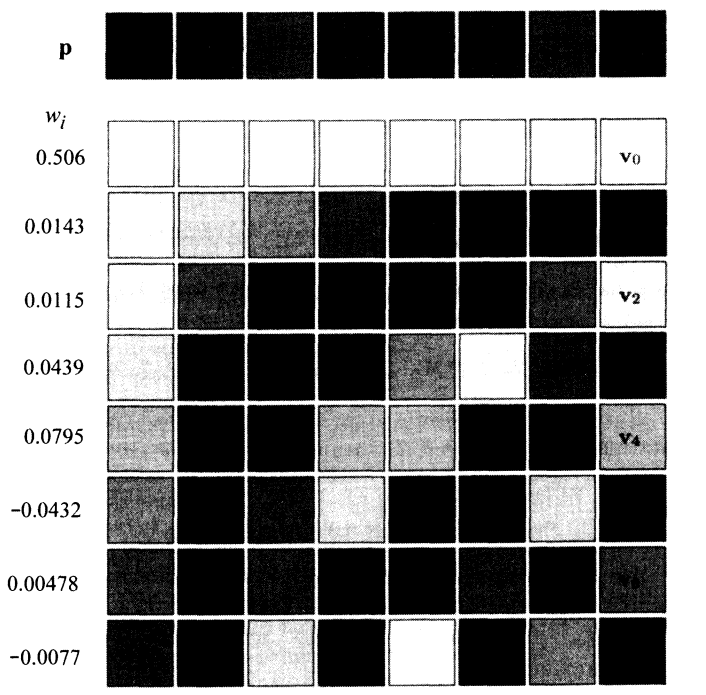
\includegraphics[width=0.7\textwidth]{/home/evgen/Coursework/app/diplom/images/grap_prew_dct.png}
    \caption{Графическое представление одномерного DCT.}
    \label{fig:gr_dt}
\end{figure}

\clearpage
Все восемь векторов $v_i$ показаны в виде ряда из восьми маленьких серых квадратиков,
причем значение $+1$ представлено белым цветом, а значение $-1$ окрашено в ченый цвет. 
Каждый из восьми компонентов вектора $p$ выражен в виде взвешенной суммы восьми серых оттенков.

На практике одномерное DCT проще всего вычислять по формуле

\begin{equation}
    G_f = \frac{1}{2}C_f \sum_{t=0}^{7} p_t \cos{\frac{(2t+1)f \pi}{16}}
    \label{eq:dct}
\end{equation}

$$
\quad \text{где} \quad C_f = 
\left\{
    \begin{array}{ll}
        \frac{1}{\sqrt{2}}, & f = 0, \\
        1, & f > 0. 
    \end{array}
\right.
\quad \text{При} \quad f = 0, 1, \dots, 7.
$$


Здесь исходными данными (пикселами, фрагментами звука или дру­гими элементами) являются величины $p_t$, 
а им соответствующими коэффициентами DCT служат числа $G_f$. 
Формула \eqref{eq:dct} очень про­ста, но процесс вычисления по ней медленный. 
Декодер получает на входе ко­эффициенты DCT, делит их на восьмерки и применяет к ним обрат­ное преобразование DCT (inverse DCT, IDCT) 
для восстановления исходных данных (тоже в виде групп по 8 элементов). Простейшая формула для вычисления IDCT имеет вид

\begin{equation}
    p_t = \frac{1}{2} \sum_{j=0}^{7} C_j G_j \cos{\frac{(2t+1)j \pi}{16}, \text{при} \; t = 0,1, \dots, 7}
\end{equation}


%%%%%%%%%%%%%%%%%%%%%%%%%%%%%%%%%%%%%%%%%%%%%%
\subsection{Двумерное (матричное) DCT}

Из опыта хорошо известно, что пикселы изображения имеют корреляцию  не только по горизонтали, но и по вертикали. 
То есть пиксели взаимосвязаны как с соседними пикселами слева и справа, так и с пикселами сверху и снизу. 
Поэтому методы сжатия изо­бражений используют двумерное DCT, которое задается формулой

\begin{equation}
    G_{ij} = \frac{1}{\sqrt{2n}} C_i C_j\sum_{x=0}^{n-1} \sum_{y=0}^{n-1} p_{xy} \cos{\frac{(2y+1)j \pi}{2n} \cos{\frac{(2x+1)i \pi}{2n}}}
    \label{eq:2D_DCT}
\end{equation}


Для каждого коэффициента $G_{ij}$ необходимо выполнить две вложенные суммы по $n$ элементам, 
что даёт вычислительную сложность $O(n^2)$ на один коэффициент. 
Поскольку всего коэффициентов $n^2$, общая сложность для наивного вычисления двумерного DCT равна:

\begin{equation}
    O(n^2) \times O(n^2) = O(n^4)
    \label{eq:asimp_dct}
\end{equation}


Использование алгоритмов быстрого дискретного косинус-преобразования (Fast DCT), 
аналогично быстрому преобразованию Фурье (FFT), 
позволяет дополнительно снизить вычислительную сложность одномерного DCT с $O(n^2)$ до $O(n \log{n})$.
В таком случае двухмерное DCT реализуется как две последовательные одномерные операции, и общая сложность становится:

\begin{equation}
    O(n \log{n})
    \label{eq:fast_asimp_dct}
\end{equation}


при $0 \leq i, j \leq n - 1$. Изображение разбивается на блоки пикселов $p_{xy}$ размера $n \times n$ (в данном примере $n = 8$), 
и уравнение \eqref{eq:2D_DCT} используется для нахождения коэффициентов $G_{ij}$ для каждого блока пикселов.
Если частичная потеря информации допустима, то коэффициенты подвергаются квантованию, что будет подробно рассмотрено в следующем разделе. 
Декодер восстанавливает сжатый блок данных (точно или приближенно), вычисляя обратное DCT (IDCT) по формуле


\begin{equation}
    p_{xy} = \frac{1}{4} \sum_{i = 0}^{7} \sum_{j = 0}^{7} C_i C_j G_{ij} \cos{\frac{(2y+1)j \pi}{16} \cos{\frac{(2x+1)i \pi}{16}}}
    \label{eq:I2D_DCT}
\end{equation}

$$
\quad \text{где} \quad C_f = 
\left\{
    \begin{array}{ll}
        \frac{1}{\sqrt{2}}, & f = 0, \\
        1, & f > 0. 
    \end{array}
\right.
$$


Двумерное дискретное косинусное преобразование (DCT) можно интерпретировать двумя способами: как композицию двух вращений, 
а также через представление вектора в базисе $n$-мерного векторного пространства. 
В первой ин­терпретации используется блок $n \times n$ пикселов (рис. \eqref{fig:coefs}a, где элементы обозначены буквой "L")


\begin{figure}[h!]
    \centering
    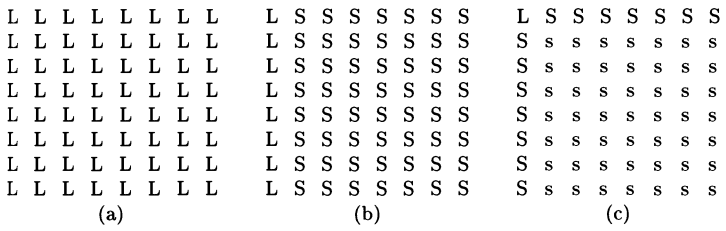
\includegraphics[width=0.7\textwidth]{/home/evgen/Coursework/app/diplom/images/coef_blocks.png}
    \caption{Двумерное DCT и двойное вращение.}
    \label{fig:coefs}
\end{figure}


Сначала рассматриваются строки этого блока как точки $(p_{x,0}, p_{x,1}, \dots, p_{x,n-1})$ в $n$- мерном пространстве,
которые поворачиваются в этом пространстве с помощью преобразования, задаваемого внутренней суммой

$$
G1_{x,j} = C_j \sum_{y=0}^{n-1} p_{xy} \cos{\frac{(2y+1)j \pi}{2n}}
$$


из уравнения \eqref{eq:2D_DCT}. Результатом этого вращения служит блок $G1_{x,j}$ из $n \times n$ коэффициентов, 
в котором в строках доминируют первые элементы (обозначенные как «L» на рис. \eqref{fig:coefs}b), 
в то время как все остальные элементы малы (они обозначены как «S»). Внешняя сумма, приведенная в уравнении \eqref{eq:2D_DCT}, равна


$$
G_{ij} = \frac{1}{\sqrt{2n}} C_i \sum_{x=0}^{n-1} p_{xy} G1_{x,j} \cos{\frac{(2x+1)i \pi}{2n}}
$$

Здесь уже столбцы матрицы $1_{x,j}$ рассматриваются в качестве то­чек $n$ - мерного векторного пространства, над которыми совершает­ся преобразование вращения. 
В результате получается один боль­шой коэффициент в верхнем левом углу блока (на рис.\eqref{fig:coefs}c - это «L») 
и $N^2 - 1$ маленьких коэффициентов в остальных местах («S» и «s» на рисунке). 
Эта интерпретация рассматривает двумерное DTC в виде двух разных вращений размерности $n$. 


Вторая интерпретация (при $n = 8$) использует уравнение \eqref{eq:2D_DCT} для создания 64 блоков по $8 \times 8$ величин в каждом. 
Все 64 блока рас­сматриваются в качестве базиса 64-мерного векторного простран­ства (это базисные изображения). 
Любой блок $B$ из $8 \times 8$ пикселов можно выразить как линейную комбинацию этих базисных изобра­жений, 
и все 64 веса этой линейной комбинации образуют коэффи­циенты DCT блока $B$.


\begin{figure}[h!]
    \centering
    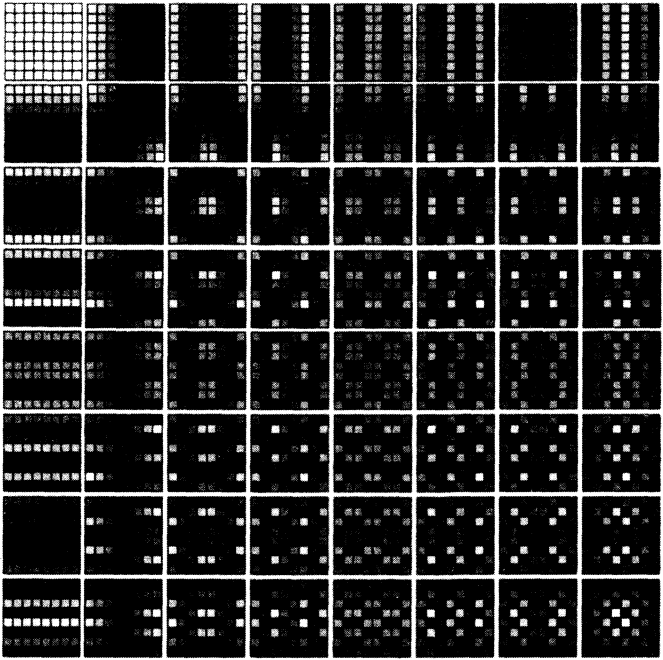
\includegraphics[width=0.7\textwidth]{/home/evgen/Coursework/app/diplom/images/basis2dDCT.png}
    \caption{64 базисных изображения двумерного DCT.}
    \label{fig:basis2dDCT}
\end{figure}


На рисунке выше представлено графическое отображение 64 базисных функций 
двумерного дискретного косинусного преобразования (DCT) при размере блока $n=8$.
 Каждый элемент с координатами $(i,j)$ на данном рисунке соответствует блоку размером $8 \times 8$, 
 полученному в результате вычисления выражения $\cos{(i \cdot s)} \cdot \cos{(j \cdot t)}$, 
 где переменные $s$ и $t$ изменяются независимо в пределах, определённых уравнением \eqref{eq:theta_values}.\\


 Подведем итог этого, довольно сложного шага. Сжатие любого изображения с помощью DCT можно теперь сделать следующим образом.


 \begin{enumerate}
    \item Разделить изображение на $k$ блоков пикселов размером $n \times n$ (чаще всего используется размер $8 \times 8)$.
    \item Применить дискретное косинусное преобразование (DCT) к каждому блоку $B^{(i)}$, представив его в виде линейной комбинации
    64 базисных функций, показанных на рисунке выше. В результате получится набор блоков (далее будем называть их векторами) $W^{(i)}$,
    каждый из которых содержит 64 коэффициента $\omega^{(i)}_{j}$, где $j = 0, 1, \dots, 63$.
    \item Векторы $W^{(i)}$, где $i = 1, 2, \dots, k$, группируются по компонентам, формируя 64 отдельных вектора коэффициентов
    $$
    \mathbf{C_j} = \{ \omega^{(1)}_j, \omega^{(2)}_j, \dots, \omega^{(k)}_j \}.
    $$
    В частности, вектор $\mathbf{C_0}$ состоит из $k$ коэффициентов DC.
    \item Каждый вектор коэффициентов $C^{(j)}$ подвергается квантованию независимо от остальных. 
    Полученные квантованные векторы $Q^{(j)}$ далее могут быть дополнительно сжаты с использованием методов, 
    таких как RLE, код Хаффмана или других алгоритмов, и записаны в сжатый файл.
 \end{enumerate}



%%%%%%%%%%%%%%%%%%%%%%%%%%%%%%%%%%%%%%%%%%%%%%
\subsection{Квантование}

В процессе сжатия изображений важным этапом является \textbf{квантование}, 
под которым понимается преобразование чисел с высокой точностью (чаще всего вещественных) в значения с меньшей точностью, 
например — округление до ближайшего целого или замена на приближённое значение из ограниченного набора. 

Это позволяет существенно уменьшить объём передаваемой или сохраняемой информации за счёт исключения наименее значимых деталей, 
воспринимаемых человеком слабо либо вовсе незаметных.

Существует два основных подхода к квантованию — \textbf{скалярное} и \textbf{векторное}.

\textbf{Скалярное} квантование представляет собой поэлементную обработку данных, 
когда каждое значение преобразуется независимо от других. 
Этот метод прост в реализации и интуитивно понятен, но не всегда обеспечивает оптимальный результат: 
полезная информация может быть утеряна даже в значимых фрагментах, если не учитывать взаимосвязь между соседними значениями.

Для повышения эффективности используется \textbf{векторное} квантование, где обрабатываются не отдельные числа, 
а целые блоки данных — группы пикселей, которые рассматриваются как многомерные векторы. 
Перед началом сжатия формируется специальный набор типовых блоков — кодовая книга. 
Каждый блок изображения сравнивается со всеми элементами этой книги, и выбирается наиболее близкий (в смысле минимальной разности значений). 
Вместо самого блока в выходной поток данных записывается лишь индекс (или указатель) соответствующего эталонного блока из кодовой книги.

Поскольку индекс, как правило, занимает меньше места, чем полный блок, такой подход позволяет добиться существенного уменьшения размера изображения. 
При этом достигается разумный баланс между степенью сжатия и качеством восстановления, 
особенно если кодовая книга заранее адаптирована под характеристики изображений, с которыми предполагается работать.

В стандарте JPEG реализовано канально-зависимое скалярное квантование, при котором каждый коэффициент, 
полученный в результате дискретного косинусного преобразования (DCT), квантуется независимо от остальных. 
Для каждого из цветовых компонентов — яркостного ($Y$) и двух хроминансных ($Cb$ и $Cr$) — применяются отдельные квантовочные матрицы, 
отражающие различную чувствительность человеческого зрения к яркости и цвету. Производится простая операция 
округления или деления на фиксированный квантовочный коэффициент. Временная сложность такого подхода $O(n^2)$.
Эти матрицы сформированы на основе психовизуальных моделей и оптимизированы так, 
чтобы минимизировать визуально заметные искажения при сжатии.


\YQuantize

\CbCrQuantize

Избыточное квантование может привести к появлению блочных артефактов, особенно при низком битрейте. 
Эти артефакты возникают из-за чрезмерной потери информации в результатах квантования и часто становятся заметными на границах блоков.

Когда коэффициенты в матрице квантования слишком велики (например, при слишком сильном сжатии), 
значительная часть информации теряется, особенно в высокочастотных компонентах, которые отвечают за детали изображения. 
Этот процесс квантования приводит к значительным потерям точности в преобразованных данных. 
На изображении это выражается в виде артефактов, которые часто становятся видимыми в местах стыка блоков.

Однако, такого эффекта можно добитья и при слишком малом квантовании.
На границах блоков, где алгоритм не может точно передать информацию, 
начинается видимый переход между различными уровнями яркости или цвета, 
что приводит к образованию четких линий или квадратных паттернов, которые визуально ощущаются как артефакты.

Так же, поскольку изображение разбивается на блоки размером $8 \times 8$ пикселей, и каждый блок сжимается независимо. 
Это может привести к потере контекста между блоками, особенно в случае сильного сжатия. 
Границы блоков не могут быть плавными, из-за чего возникают резкие переходы между блоками.

Эти артефакты могут выглядеть как "ступеньки" или резкие изменения яркости и цвета, которые не присутствуют в исходном изображении.

\subsubsection{Как уменьшить блочные артефакты}

Существует несколько подходов для минимизации блочных артефактов при сжатии JPEG:
\begin{enumerate}
    \item Использование более низкого коэффициента сжатия: Уменьшение уровня сжатия помогает сохранить больше данных, 
    что уменьшает квантование и, соответственно, количество потерь информации. 
    Это снижает вероятность появления артефактов, но увеличивает размер файла.

    \item Адаптивное квантование: В некоторых случаях используется адаптивное квантование, 
    при котором для разных частей изображения выбираются различные матрицы квантования в зависимости от содержания. 
    Например, для областей с высокой детализацией можно использовать более точное квантование, а для равномерных областей — более грубое.

    \item Эксперименты с постобработкой: В некоторых случаях для устранения артефактов применяются методы постобработки, такие как сглаживание или фильтрация на уровне блоков.

    \item Использование более сложных алгоритмов сжатия: Алгоритмы сжатия, такие как JPEG2000, 
    используют более сложные методы, которые могут уменьшить или полностью устранить блочные артефакты. 
    В частности, JPEG2000 использует вейвлет-преобразования вместо DCT, что позволяет избежать проблемы разделения изображения на блоки и улучшить качество сжатия.
\end{enumerate}

\vspace{1em}

JPEG не использует векторное квантование в силу его значительно большей вычислительной и алгоритмической сложности: 
построение и оптимизация кодовой книги требуют значительных ресурсов, 
а сам процесс кодирования с подбором ближайшего эталона становится существенно менее эффективным для реализации в массовых форматах хранения изображений. 
Кроме того, векторное квантование хуже адаптируется к переменной структуре изображений и менее совместимо с блочной природой DCT-представления.




%%%%%%%%%%%%%%%%%%%%%%%%%%%%%%%%%
\subsection{Зигзаг-преобразование блоков}

После применения DCT, и последующего квантования блоков, изображение представляется в виде матрицы коэффициентов $8 \times 8$, 
где каждый коэффициент представляет собой степень различной частоты. 
Эти коэффициенты могут включать как высокочастотные (мелкие детали изображения), так и низкочастотные компоненты (общие очертания). 
Важным моментом является то, что после квантования высокочастотные коэффициенты, как правило, имеют значения, близкие к нулю, 
и не играют значительной роли для восприятия изображения. 
Поэтому их можно исключить или закодировать с меньшей точностью.

Зигзаг-преобразование используется для того, чтобы упорядочить эти коэффициенты в порядке, 
который позволяет более эффективно их кодировать. 
Суть метода в том, что он позволяет собирать все нулевые значения (или значения, близкие к нулю) в конец последовательности, 
что снижает объем данных при их дальнейшем кодировании.

Зигзаг-преобразование упорядочивает эти коэффициенты таким образом, что сначала идут наиболее значимые коэффициенты (низкочастотные), 
а затем — менее значимые (высокочастотные, которые в основном равны нулю).

Зигзагообразный порядок включает следующие шаги:

\begin{enumerate}
    \item Начинается с первого элемента в верхнем левом углу матрицы (нулевой индекс).
    \item Затем происходит движение по диагоналям матрицы, начиная с верхней левой части, последовательно переходя к правому нижнему углу.
    \item Каждая диагональ матрицы представляет собой группу коэффициентов, которые последовательно вытягиваются в одном ряду.
\end{enumerate}


\begin{figure}[h!]
    \centering
    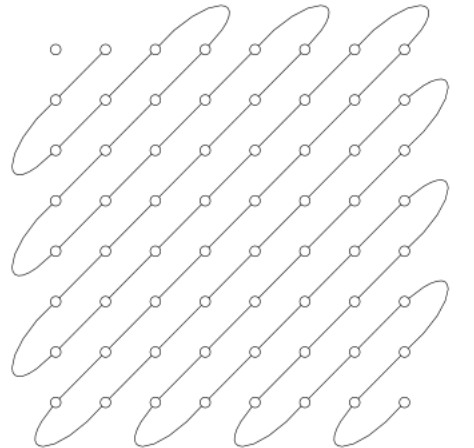
\includegraphics[width=0.7\textwidth]{/home/evgen/Coursework/app/diplom/images/zig_zag.png}
    \caption{Обход блока зиг-заг.}
    \label{fig:zig_zag}
\end{figure}


В результате применения зигзагообразного обхода к блоку преобразованных коэффициентов 
дискретного косинусного преобразования формируется линейная последовательность. Один из примеров такой последовательности приведён ниже.

\begin{equation}
    \label{eq:zigzag_example}
    \text{Последовательность после зигзагообразного обхода: } 
    \left\{
    \begin{array}{cccccccc}
    52 & -3 & 0 & 0 & 0 & 2 & 0 & 0 \\
    0 & 0 & 0 & 0 & 0 & 0 & 1 & 0
    \end{array}
    \right\}
    \end{equation}

Здесь первый элемент (52) соответствует DC-компоненте, а последующие значения — коэффициенты высоких частот (AC-компоненты), 
отсортированные по убыванию их вклада в общее изображение.


%%%%%%%%%%%%%%%%%%%%%%%%%%%%%%%%%
\subsection{RLE-кодирование}


После применения зигзаг-преобразования каждый блок коэффициентов преобразуется в одномерный массив, 
в котором значимая информация (низкочастотные коэффициенты) сосредоточена в начале, 
а большая часть оставшихся элементов принимает нулевое значение. 
Это делает полученную последовательность особенно удобной для дальнейшего сжатия с использованием методов, 
предназначенных для работы с повторяющимися элементами.

На этом этапе в классическом алгоритме JPEG традиционно применяется энтропийное кодирование, 
наиболее часто — с использованием кода Хаффмана, 
позволяющего достичь высокой степени сжатия за счёт построения оптимального префиксного кодового дерева, 
основанного на вероятностях появления различных значений. 
Однако реализация эффективного кодировщика Хаффмана требует значительных трудозатрат, 
включая построение статистической модели, генерацию кодовых деревьев и реализацию соответствующего декодирования.

В рамках данной работы энтропийное кодирование было намеренно опущено. 
Вместо него используется более простой и наглядный метод кодирования с повторениями — Run-Length Encoding (RLE), 
который позволяет проиллюстрировать фундаментальные принципы постобработки данных после зигзаг-преобразования и обеспечивает компрессию, 
достаточную для демонстрации эффективности базового JPEG-подобного сжатия. 
Это решение продиктовано необходимостью сосредоточиться на ключевых этапах сжатия и ограниченностью временных ресурсов, 
отведённых на реализацию дипломного проекта.

Применение RLE особенно эффективно в контексте JPEG-подобного представления данных, 
так как вследствие квантования и зигзагообразного упорядочивания большинство коэффициентов в конце последовательности равны нулю.
Алгоритм RLE преобразует такие повторы в компактную форму, 
заменяя длинные последовательности одинаковых значений (в первую очередь нулей) парой «значение–длина повтора», 
что существенно снижает объём итоговых данных. Временная сложность алгоритма $O(N)$, 
где N — длина последовательности (в данном случае 64).

Таким образом, хотя в полномасштабной реализации алгоритма JPEG предпочтительно использовать энтропийное кодирование, 
в рамках данной работы RLE выступает как более простая альтернатива, 
позволяющая сохранить общий принцип компрессии без существенного увеличения сложности реализации.


\begin{RLETable}
\end{RLETable}


\begin{RLEEncodedTable}
\end{RLEEncodedTable}


Применение RLE позволяет существенно сократить объём информации, подлежащей сохранению или передаче, 
при этом сохраняя возможность точного восстановления исходной последовательности. 
Хотя степень сжатия, достигаемая с помощью RLE, уступает алгоритмам энтропийного кодирования (таким как Хаффман), 
его простота и наглядность делают его отличным выбором для учебных и демонстрационных целей.

Таким образом, использование RLE в данной работе позволило реализовать полный цикл JPEG-подобного сжатия — от разделения изображения 
на блоки и применения косинус-преобразования до финального этапа кодирования, — при этом сосредоточившись на ключевых принципах без 
чрезмерного усложнения алгоритма.



%%%%%%%%%%%%%%%%%%%%%%%%%%%%%%%%%%%%%%%%%%%%%%%%%%%
\subsection{Декодирование}

Процесс декодирования JPEG является обратной операцией по отношению к этапам кодирования
и направлен на восстановление изображения из сжатого представления. 
На выходе должен быть получен массив пикселей, максимально приближенный к исходному изображению. 
Процесс декодирования включает следующие этапы:

 
\subsubsection{Распаковка закодированных данных}

На первом этапе декодирования выполняется извлечение и интерпретация сжатых данных, 
полученных после применения метода RLE (run-length encoding, кодирование длин серий). 
В процессе кодирования многие коэффициенты DCT, особенно высокочастотные, равны нулю. 
Это свойство используется для повышения степени сжатия — нули заменяются на пары вида (количество нулей, ненулевое значение).

При декодировании производится восстановление полного набора коэффициентов блока размером $8 \times 8$
из такой сжатой последовательности. Например, последовательность:

\begin{equation}
    \label{eq:rle_example}
    \begin{aligned}
        &\text{Сжатая последовательность пар (количество нулей, значение):} \\
        &\qquad (0,\ 52),\ (0,\ -3),\ (3,\ 2),\ (9,\ 1) \\
        &\text{После распаковки:} \\
        &\qquad 52,\ -3,\ 0,\ 0,\ 0,\ 2,\ 0,\ 0,\ 0,\ 0,\ 0,\ 0,\ 0,\ 0,\ 1,\ 0
    \end{aligned}
\end{equation}



\subsubsection{Обратный зигзагообразный обход}
Поскольку в процессе кодирования двумерный массив коэффициентов представлялся в виде одномерного массива 
с помощью зигзагообразного обхода, теперь необходимо восстановить исходное расположение коэффициентов в блоке $8 \times 8$. 
Каждому элементу последовательности возвращается его позиция в соответствии со стандартной зигзагообразной схемой.




\subsubsection{Обратное квантование}
На этапе обратного квантования каждый коэффициент умножается на соответствующее значение из таблицы квантования, 
использованной при кодировании. Если обозначить квантованный коэффициент как $Q_{i,j}$, а таблицу квантования как $T_{i,j}$,
то восстановленный DCT-коэффициент можно получить по формуле:

\begin{equation}
    D_{i,j} = Q_{i,j} \circ T_{i,j}
\end{equation}

Это приближает коэффициенты к их исходным значениям до потери точности при квантовании.




\subsubsection{Обратное дискретное косинусное преобразование (IDCT)}
На этом этапе выполняется обратное дискретное косинусное преобразование (IDCT) для каждого блока. 
Восстановление значений пикселей в пространственной области осуществляется на основе 64 DCT-коэффициентов, по формуле \eqref{eq:I2D_DCT}.


\subsubsection{Восстановление блоков}
После применения IDCT к каждому блоку получаются блоки из 64 значений интенсивности, которые собираются в итоговое изображение. 
При этом важно точно соблюсти позиционирование блоков и границы изображения.

После этого идет обратное преобразование цветного пространства из $\textbf{YCbCr}$ в $\textbf{RGB}$, 
что позволяет получить восстановленное изображение в привычном для восприятия формате.

% Однако, несмотря на сложность и точность процесса декодирования, JPEG не всегда идеален для всех типов изображений. 
% Алгоритм сжатия может проявлять свои ограничения, 
% особенно в случае с изображениями с ярко выраженными границами и резкими переходами, где заметны артефакты, 
% такие как блоковые искажения. 
% Эти ограничения обусловлены особенностями самого алгоритма, 
% который оптимизирован для сжатия изображений с плавными переходами и небольшими деталями, 
% но может не справляться с сохранением чёткости на изображениях с высококонтрастными зонами.

% Таким образом, несмотря на высокую эффективность JPEG и его широкое распространение, 
% в специфических случаях, таких как изображения с четкими линиями и границами, алгоритм может показывать свои слабые стороны. 
% В таких ситуациях целесообразно использование вариации параметров на разных этапах алгоритма.
% Можно пробовать изменять коэффициент сжатия на этапе квантования или менять размер блока при разбиении.
% В некоторых случаях используется адаптивное квантование, 
% при котором для разных частей изображения выбираются разные матрицы квантования в зависимости от содержания.
% Для устранения артефактов после сжатия применяются методы постобработки, такие как сглаживание или фильтрация на уровне блоков, 
% что помогает улучшить визуальное восприятие изображения.

% Помимо этого, существуют более продвинутые алгоритмы сжатия, которые изначально ориентированы на устранение подобных недостатков. 
% Так, например, JPEG2000 использует вейвлет-преобразования вместо DCT, 
% что позволяет избежать деления изображения на независимые блоки. 
% Это снижает вероятность появления блоковых артефактов и обеспечивает более высокое качество сжатия при сопоставимом уровне потерь.